%%% LyX 2.0.5.1 created this file.  For more info, see http://www.lyx.org/.
%%% Do not edit unless you really know what you are doing.
%\documentclass[twoside,english]{report}
%\usepackage[T1]{fontenc}
%\usepackage[latin9]{inputenc}
%\setcounter{secnumdepth}{3}
%\setcounter{tocdepth}{3}
%\usepackage[active]{srcltx}
%\usepackage{verbatim}
%\usepackage{graphicx}
%\usepackage{setspace}
%\usepackage[numbers]{natbib}
%\doublespacing
%
%\makeatletter
%
%\makeatother
%
%\usepackage{babel}
%\begin{document}

\chapter{Background}


\section{Hand Writing Recognition}
Handwriting recognition is a task of transforming a language represented in its spatial form of graphical marks into its symbolic representation. 
At the highest level, handwriting recognition can be broken into two categories: offline and online. 

\emph{TODO: Review \cite{bahlmann2005advanced} thesis}

\subsection{On-line vs. Off-line Handwriting Recognition}
\emph{see: \cite{al2010development} section "types of handwriting input - on-line and off-line"}
While much of the today's data is directly entered into computers using the keyboard, many tasks still exist in which people tend to prefer handwriting over keyboard entry. Note taking (e.g. in classrooms) is a task that can still be done more efficiently by hand for most users. In addition, while people can produce annotated hand sketches very quickly, data entry into a computer using a combination of the mouse and keyboard is relatively time consuming\cite{connell2000online}.
Smartphones and tablets are pocket sized consumer devices that can store calendars and address books, provide access to emails, the web, and contain other productivity tools. These devices are too small to have full sized keyboards, or sometimes may be too small for any keyboard at all, requiring pen, hand gestures, figure gestures or voice interface to enter data \cite{connell2000online}. 
The problem of handwriting recognition has now been a topic of research for over four decades. There are many types of problems (with varying complexity) within handwriting recognition, based on how the data is presented to the recognition system, at what level the data can be unambiguously broke n into pieces (e.g. individual characters or words), and the transcription complexity of the language used \cite{connell2000online}. 
Offline handwriting recognition focuses on documents that have been written on paper at some previous point of time. Information is presented to the system in the form of scanned image of the paper document. In contrast, online Hand Writing Recognition refers to the situation where the recognition is performed concurrently to the writing process. This requires the use of special equipment, such touch screen or digitizing tablet, to capture the strokes of the pen as that are being written. The trace of a writer's pen is stored as a sequence of points sampled at equally spaced time intervals. The information captured for each sample is the   coordinates. While this sequence can be used to construct a static image of the writing, thus allowing offline character recognition techniques to be applied, it has been shown that the information about the pen dynamics can be used to obtain a better recognition accuracies than the static data alone. Therefore, it is beneficial to capture the data in an online form, even if the real-time processing requirements can be relaxed \cite{connell2000online}. 
Another advantage of online handwritten data over offline data is the availability of the stroke segmentation and the order of writing. Ink in static images must first be separated from the image background, creating a potential source of error. The ability to detect the states of "pen-down" (when the pen touches the tablet or the finger touches the touch screen) and "pen-up" can also be used. A single stroke is defined as the sequence of sample points occurring between consecutive pen-down and pen-up transitions. However, a complication occurs when a stroke is added to a character in a word after the rest of the word has already been written, such as the cross of a 't' or an 'x', or the dot of an 'i' or a 'j' These types are called delayed strokes \cite{connell2000online}. 

{\color{blue}Handwriting data is converted to digital form either by
scanning the writing on paper or by writing with a special
pen on an electronic surface such as a digitizer combined
with a liquid crystal display. The two approaches are
distinguished as off-line and on-line handwriting, respectively.
In the on-line case, the two-dimensional coordinates
of successive points of the writing as a function of time are
stored in order, i.e., the order of strokes made by the writer
is readily available. In the off-line case, only the completed
writing is available as an image. The on-line case deals with
a spatio-temporal representation of the input, whereas the
off-line case involves analysis of the spatio-luminance of an
image. Fig. 1 shows typical input signals that can be
analyzed in both cases. The raw data storage requirements are widely different. The data requirements for an average
cursively written word are: in the on-line case (Fig. 1b), a
few hundred bytes, typically sampled at 100 samples per
second, and in the off-line case (Fig. 1a), a few-hundred
kilo-bytes, typically sampled at 300 dots per inch. From a
global perspective, paper documents, which are an inherently
analog medium, can be converted into digital form by
a process of scanning and digitization. This process yields a
digital image. For instance, a typical 8.5 x 11 inch page is
scanned at a resolution of 300 dots per inch to create a grayscale
image of 8.4 megabytes. The resolution is dependent
on the smallest font size that needs reliable recognition, as
well as the bandwidth needed for transmission and storage
of the image. \cite{plamondon2000online}}

\begin{figure}
	\centering
        \subfloat[]{
            \label{fig:offline}
            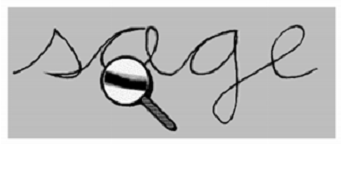
\includegraphics[width=0.5\textwidth]{./figures/offline}
        }
        \subfloat[]{
           \label{fig:online}
           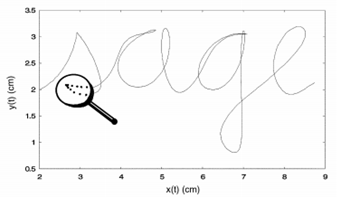
\includegraphics[width=0.5\textwidth]{./figures/online}
        }        
    \caption{(a) Off-line word. The image of the word is converted into gray-level pixels using a scanner. (b) On-line word. The x; y coordinates of the pen-tip are recorded as a function of time with a digitizer}
   \label{fig:offlibe_vs_online}
\end{figure}

\emph{talk about Writer Dependent vs. Writer Independent}

\emph{talk about Closed vs. Open Dictionary}


\section{Characteristic of the Arabic writing system}
\emph{[See Online handwriting recognition for the Arabic Letter Set]}
\emph{[See [1]	G. a. Abandah and M. Z. Khedher, "Analysis of Handwritten Arabic Letters Using Selected Feature Extraction Techniques,"International Journal of Computer Processing of Languages, vol. 22, no. 01, pp. 49-73, Mar. 2009.]}

{\color{blue}The Arabic language is one of the most structured and served languages. It comes as the fifth of the most used languages (as a first language) after Chinese, Hindi, Spanish and English. It is spoken as a first language by nearly 350 million people around the globe, mainly in the Arab countries, which is about 5.5\% of the world population (the world population is estimated at 6.44 billion in July 2005) (CIA, 2005). However, almost all Muslims (close to $1/4$ of the world population) can read Arabic script as it is the language of the Holy Qur'an. The Arabic script evolved from a type of Aramaic, with the earliest known document dating from 512 AD. The Aramaic language has fewer consonants than Arabic (Burrow, 2004). The old Arabic was written without dots or diacritics. The dots were first introduced by Yahya bin Ya'mur (died around 746 AD) and Nasr bin Asim (died around 707 AD), students of Abu Al-Aswad Al-Du'ali (died around 688 AD) who introduced the diacritics to prevent the Qur'an from being misread by Muslims (Al-Fakhri, 1997). Figure 1 shows a sample of an old manuscript of a sentence written without dots or diacritics. Due to the Islamic conquests, the use of Arabic language extended in the 7th and 8th centuries from India to the Atlantic Ocean (Al- Fakhri, 1997). Consequently, many other languages adopted the Arabic alphabet with some changes. Among those languages are Jawi, Urdu, Persian, Ottoman, Kashmiri, Punjabi, Dari, Pashto, Adighe, Baluchi, Ingush, Kazakh, Uzbek, Kyrgyz, Uygur, Sindhi, Lahnda, Hausa, Berber, Comorian, Mandinka, Wolof, Dargwa, and few others. Figure 2 shows samples of some of the above mentioned languages. However, it must be mentioned that some of those languages are currently using Latin characters, but in general, people can still read the Arabic script. It is also worth mentioning that the United Nation adopted Arabic in 1974 as its sixth official language (Strange, 1993). Despite the fact that Arabic alphabets are used in many languages, Arabic Character Recognition (ACR) has not received enough interests from researchers. Little research progress has been achieved as compared to the one done on Latin or Chinese. It has almost only started in 1975 by Nazif (1975), while the earlier research efforts in Latin may be traced back to the middle of the 1940s. However, due to a lack of computing power, no significant work was performed until the 1980s. Recent years have shown a considerable increase in the number of research papers related to ACR. (Segmentation of Arabic Characters: A Comprehensive Survey)}\\

The Arabic Aleph bet is widely used for more than twenty different languages such as Farsi, Urdu, Malay, Housa and Ottoman Turkish. Arabic is used in over 20 different countries, written by more than 100 million people and spoken by 234 million people. Although the spoken Arabic is slightly different from country to country, the written Arabic is standard system used all over the Arab world \cite{saabni2009efficient} \cite{jannoud2007automatic}.
Arabic Scripts consists of 28 basic letters, 12 additional special letters, and 8 diacritics. Arabic script is written from right to left in a semi-cursive manner in both printed and handwritten. Most letters are written in four different letter shapes depending on their position in a word, e.g., the letter \RL{`}  (Ain) appears as \RL{`} (isolated), \RL{`-}(initial),\RL{-`-} (medial) and \RL{-`} (final). Among the basic letters, six are Disconnective - \RL{A} (Alef), \RL{d} (Dal), \RL{_d} (Thal), \RL{r} (Reh), \RL{z} (Zain) and \RL{w} (Waw). Disconnective letters do not connect to the following letter and have only two shapes each. The presence of this letters interrupts the continuity of the graphic form of a word. We denote connected letters in a word, as word-part. If the word-part is composed of only one letter, this letter will be in its isolated shape \cite{biadsy2011segmentation}. 
Certain characteristics relating to the obligatory dots and strokes of the Arabic script distinguish it from Roman script, making the recognition of words in Arabic more difficult than in Roman script. First, Most Arabic letters contain dots in addition to the letter body, such as \RL{s} (Sheen) which consists of \RL{s} (Seen) body and three dots above it. In addition to dots, there are stroke that can attach to a letter body creating new letter such as \RL{k}, \RL{.t} and \RL{lA}. These dots and strokes are called delayed strokes since they are usually drawn last in the in handwritten word-part/word. Second, eliminating, adding or moving a dot or stroke could produce a completely different letter and, as a result, produce a word other than the one that was intended (see Table 1). Third, the number of possible variations of delayed strokes is greater than those in Roman scripts, as shown in Figure 2. There are only three such strokes used for English: the cross in the letter t, the slash in x, and the dots in i and j. 

{\color{blue}The Arabic language has some diacritics that are used in the holy book Qur'an and sometimes in teaching material and poetry. These diacritics are small markings used above or below the letters of a word to specify the exact pronunciation of the word. They are not commonly used in the daily, scientific, and business uses, and are not discussed further in this work.(Abandah \& Khedher, 2009)}

Finally, in Arabic script a top-down writing style called vertical ligatures is very common - letters in a word may be written above their consequent letters. In this style, the position of letters cannot be predefined relative to the baseline of the word \cite{biadsy2011segmentation}.    
Saabni and El-sana have explored a large collection of Arabic texts and extracted 300,000 different word combinations of 82,000 different word-parts. Ignoring the additional strokes reduced the number of different word-parts to 40,000 \cite{saabni2009efficient}. 

\emph{TODO: see the section "Overview of Arabic Letters" in \cite{abandah2009analysis}. It talks about letters frequencies and special letters}

\emph{TODO: talk about the WP and give statistics of WP length as described in {abandah2009analysis}}

\section{Issues of on-line handwriting recognition}
\emph{TODO: for all these sections see H. Shu, "On-line handwriting recognition using hidden Markov models," 1996.}
\subsection{Styles and Handwriting: Printed vs. Cursive}

\subsection{Writer-Dependent vs. Writer-Independent}

\subsection{Closed-Vocabulary vs, Open-Vocabulary}


\section{Arabic Handwriting Recognition}
\emph{TODO:see the in introduction of \cite{abandah2009analysis}}

\section{Issues with Arabic Handwriting Recognition}

%\end{document}
